\providecommand{\main}{../../../..}
\documentclass[\main/dresen_thesis.tex]{subfiles}
\begin{document}
  \label{sec:looselyPackedNS:nanoparticle:vsm}
  \begin{figure}[tb]
    \centering
    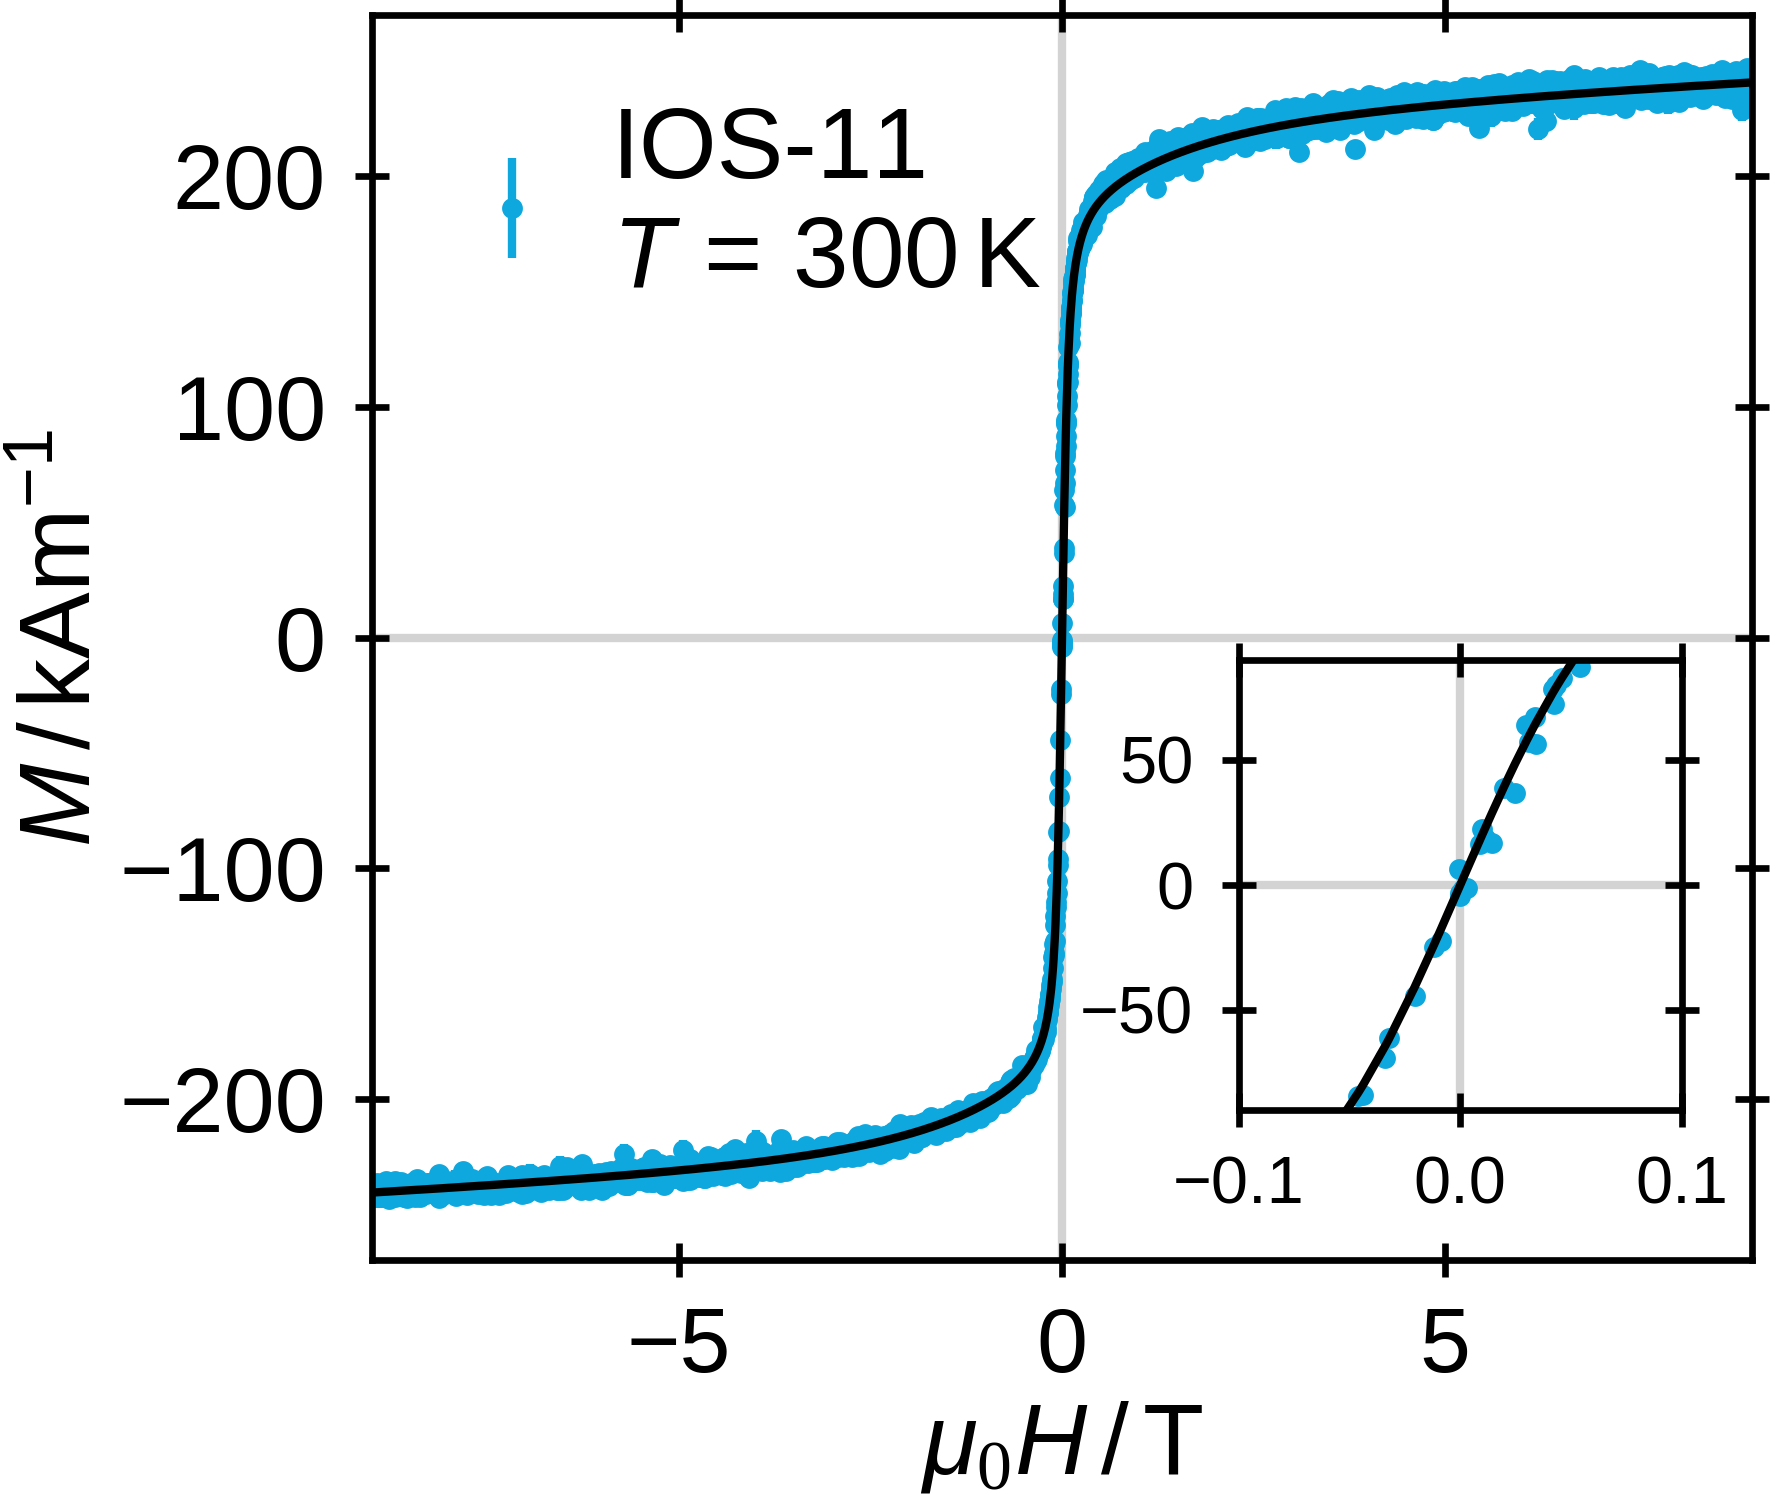
\includegraphics{looselyPackedNP_VSM_IOS-11}
    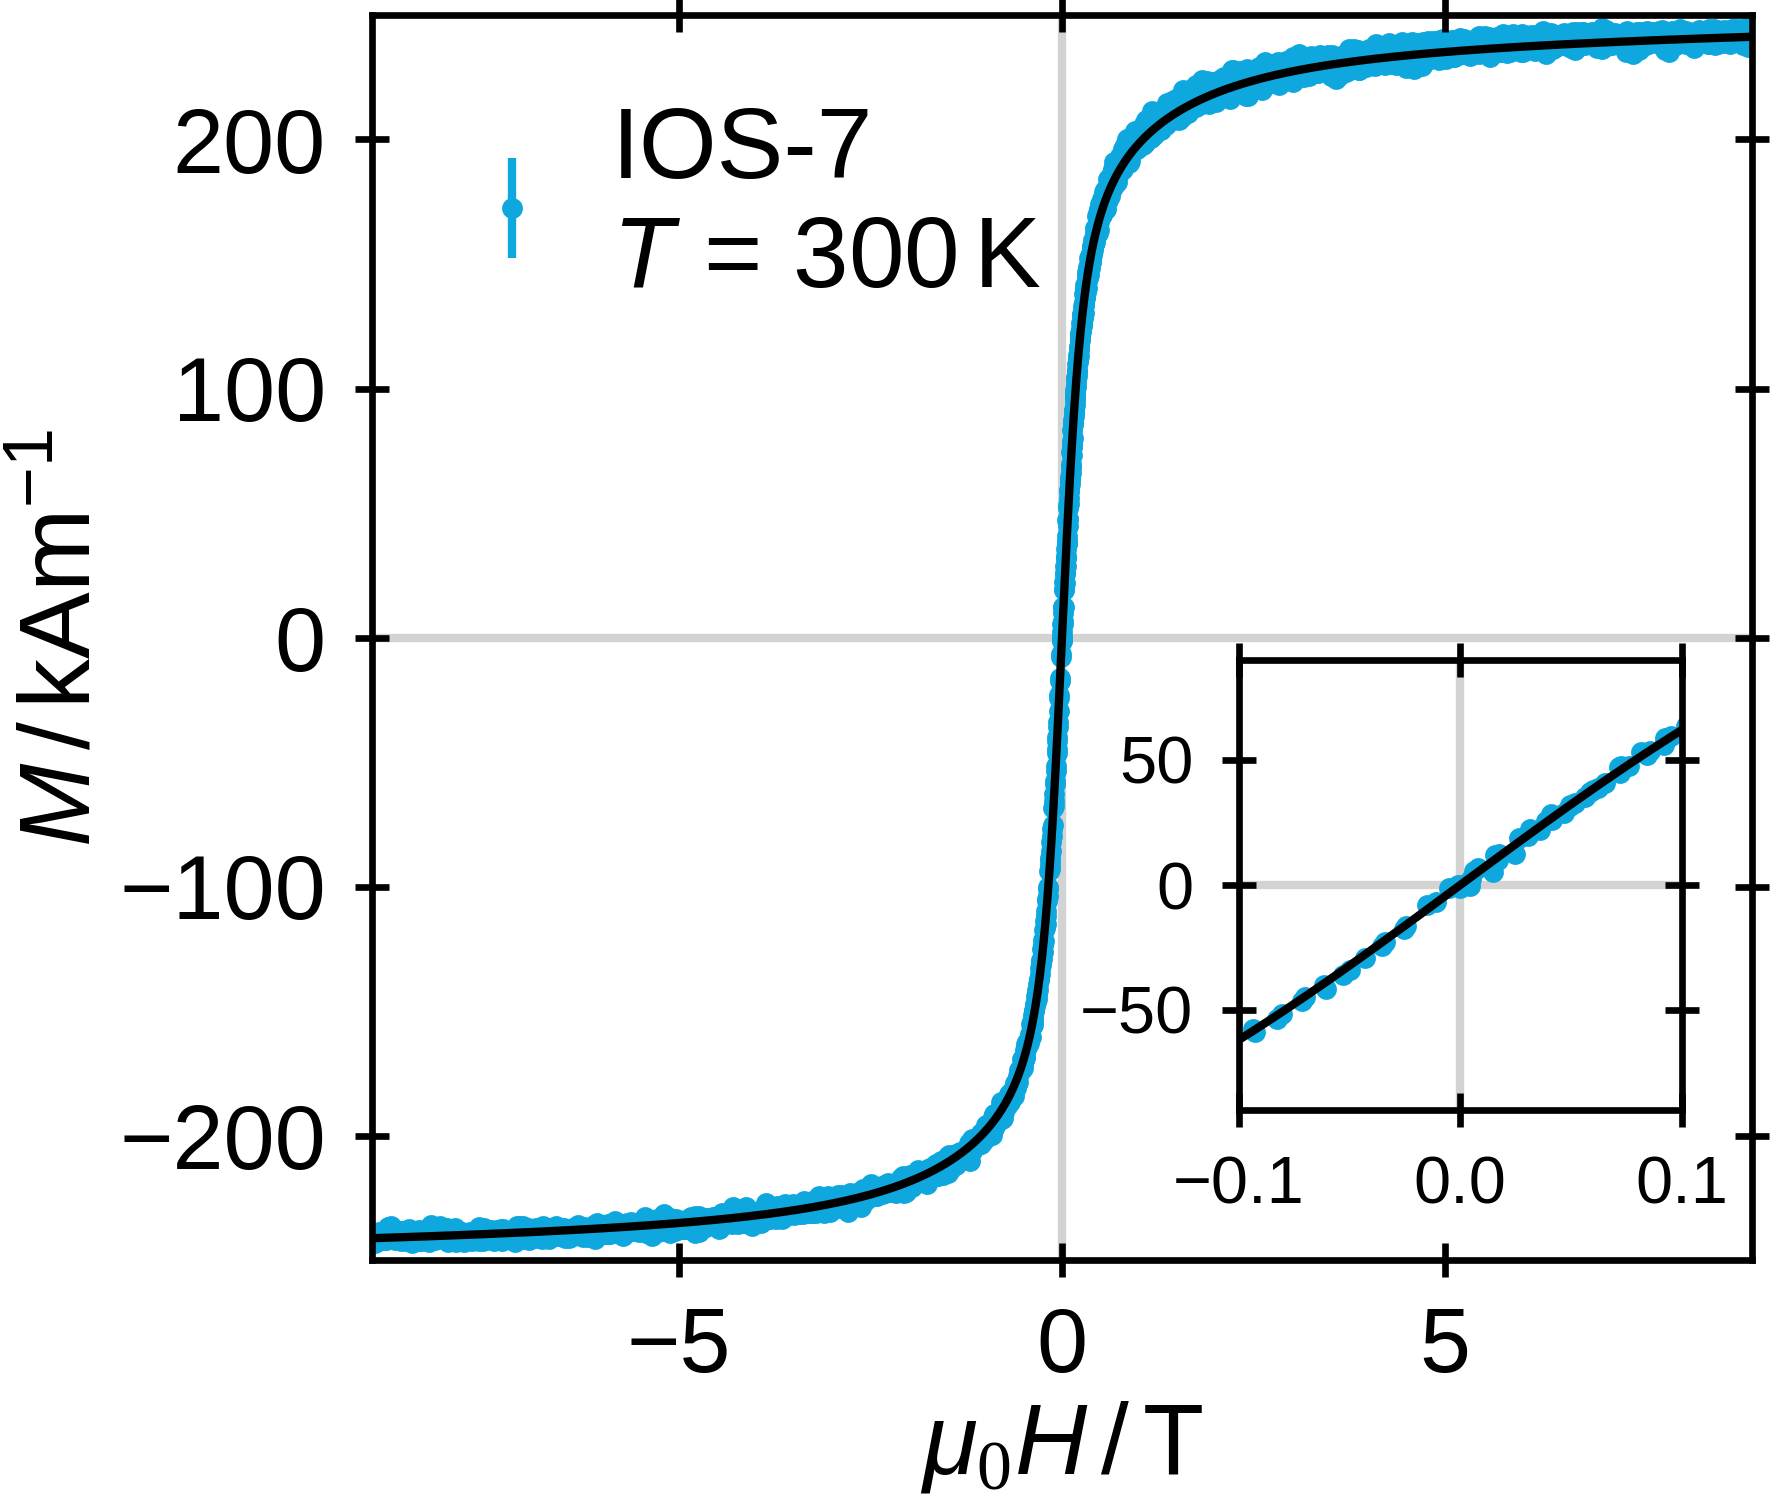
\includegraphics{looselyPackedNP_VSM_IOS-7}
    \caption{\label{fig:looselyPackedNP:nanoparticle:vsm}Room temperature vibrating sample magnetometry for IOS-11 (left) and IOS-7 (right). In black a Langevin behaviour with excess susceptibility is fit and the parameters are given in \reftab{tab:looselyPackedNP:nanoparticle:vsm}}
  \end{figure}

  Vibrating sample magnetometry is used to probe the macroscopic magnetization of IOS-11 and IOS-7.
  The measured magnetization of a dispersion at room temperature is shown in \reffig{fig:looselyPackedNP:nanoparticle:vsm}.
  In both cases a superparamagnetic behaviour is observed, which is parametrized by fitting the data with a Langevin curve and excess susceptibility.
  The parameters for the fitted magnetization curves are given in \reftab{tab:looselyPackedNP:nanoparticle:vsm}.

  \begin{table}[!htbp]
    \centering
    \caption{\label{tab:looselyPackedNP:nanoparticle:vsm}Parameters for the Langevin function with excess susceptibility shown in \reffig{fig:looselyPackedNP:nanoparticle:vsm}.}
    \begin{tabular}{ c | l | l }
      \rule{0pt}{2ex} \textbf{VSM} & IOS-11 & IOS-7 \\
      \hline
      \rule{0pt}{2ex} $M_s \, /  \unit{kAm^{-1}}$               & $164.1(1)$    & $183.2(1)$\\
      \rule{0pt}{2ex} $\mu \, / \, \mu_B$                       & $11354(58)$   & $3609(8)$\\
      \rule{0pt}{2ex} $\mu_0 \chi$                              & $0.00337(3)$  & $-0.00080(3)$\\
      \hline
      \rule{0pt}{2ex} $\chi^2$                                  & $4.8 $        & $3.3$\\
      \hline
    \end{tabular}
  \end{table}
  % \rule{0pt}{2ex} $V_\mathrm{rescale} \, / \unit{\musf L}$  & $0.0610$      & $0.0181$\\
  % \hline

  The observed saturation magnetization can be compared to the values obtained from SANSPOL.
  For IOS-11, VSM yields a magnetization of $164 \unit{kA m^{-1}}$ and from SANSPOL an average particle magnetization of $200(10)\unit{kA m^{-1}}$ has been observed.
  For IOS-7, in VSM a room temperature magnetization of $183 \unit{kA m^{-1}}$ is measured, and from SANSPOL $199\unit{kA m^{-1}}$ was obtained.
  The values from VSM are slightly smaller in comparison to SANSPOL but in a similar order of magnitude.
  A systematic error in the VSM value can be introduced from the scaling procedure of the magnetization to the particle size.
  To determine the particle magnetization in VSM, the measured data is rescaled according to the observed magnetic moment and by assuming for the magnetic particle volume the single particle volume that is obtained from SAXS.
  Thus, if the magnetic volume is actually smaller in the particle than the physical volume \eg because of a magnetically dead surface layer, the VSM values is a lower limit for the observable particle magnetization.

  The slightly larger paramagnetic excess susceptibility in IOS-11 that remains after the subtraction of the background diamagnetism hints to the w\"ustite phase within the nanoparticles.
  The signal is however too weak and in similar order of magnitude to the subtracted diamagnetic background ($\mu_0 \chi_\mathrm{bg} \eq -0.0031$) and it is therefore difficult to make quantitative claims on the w\"ustite content from the susceptibility.

  \begin{figure}[tb]
    \centering
    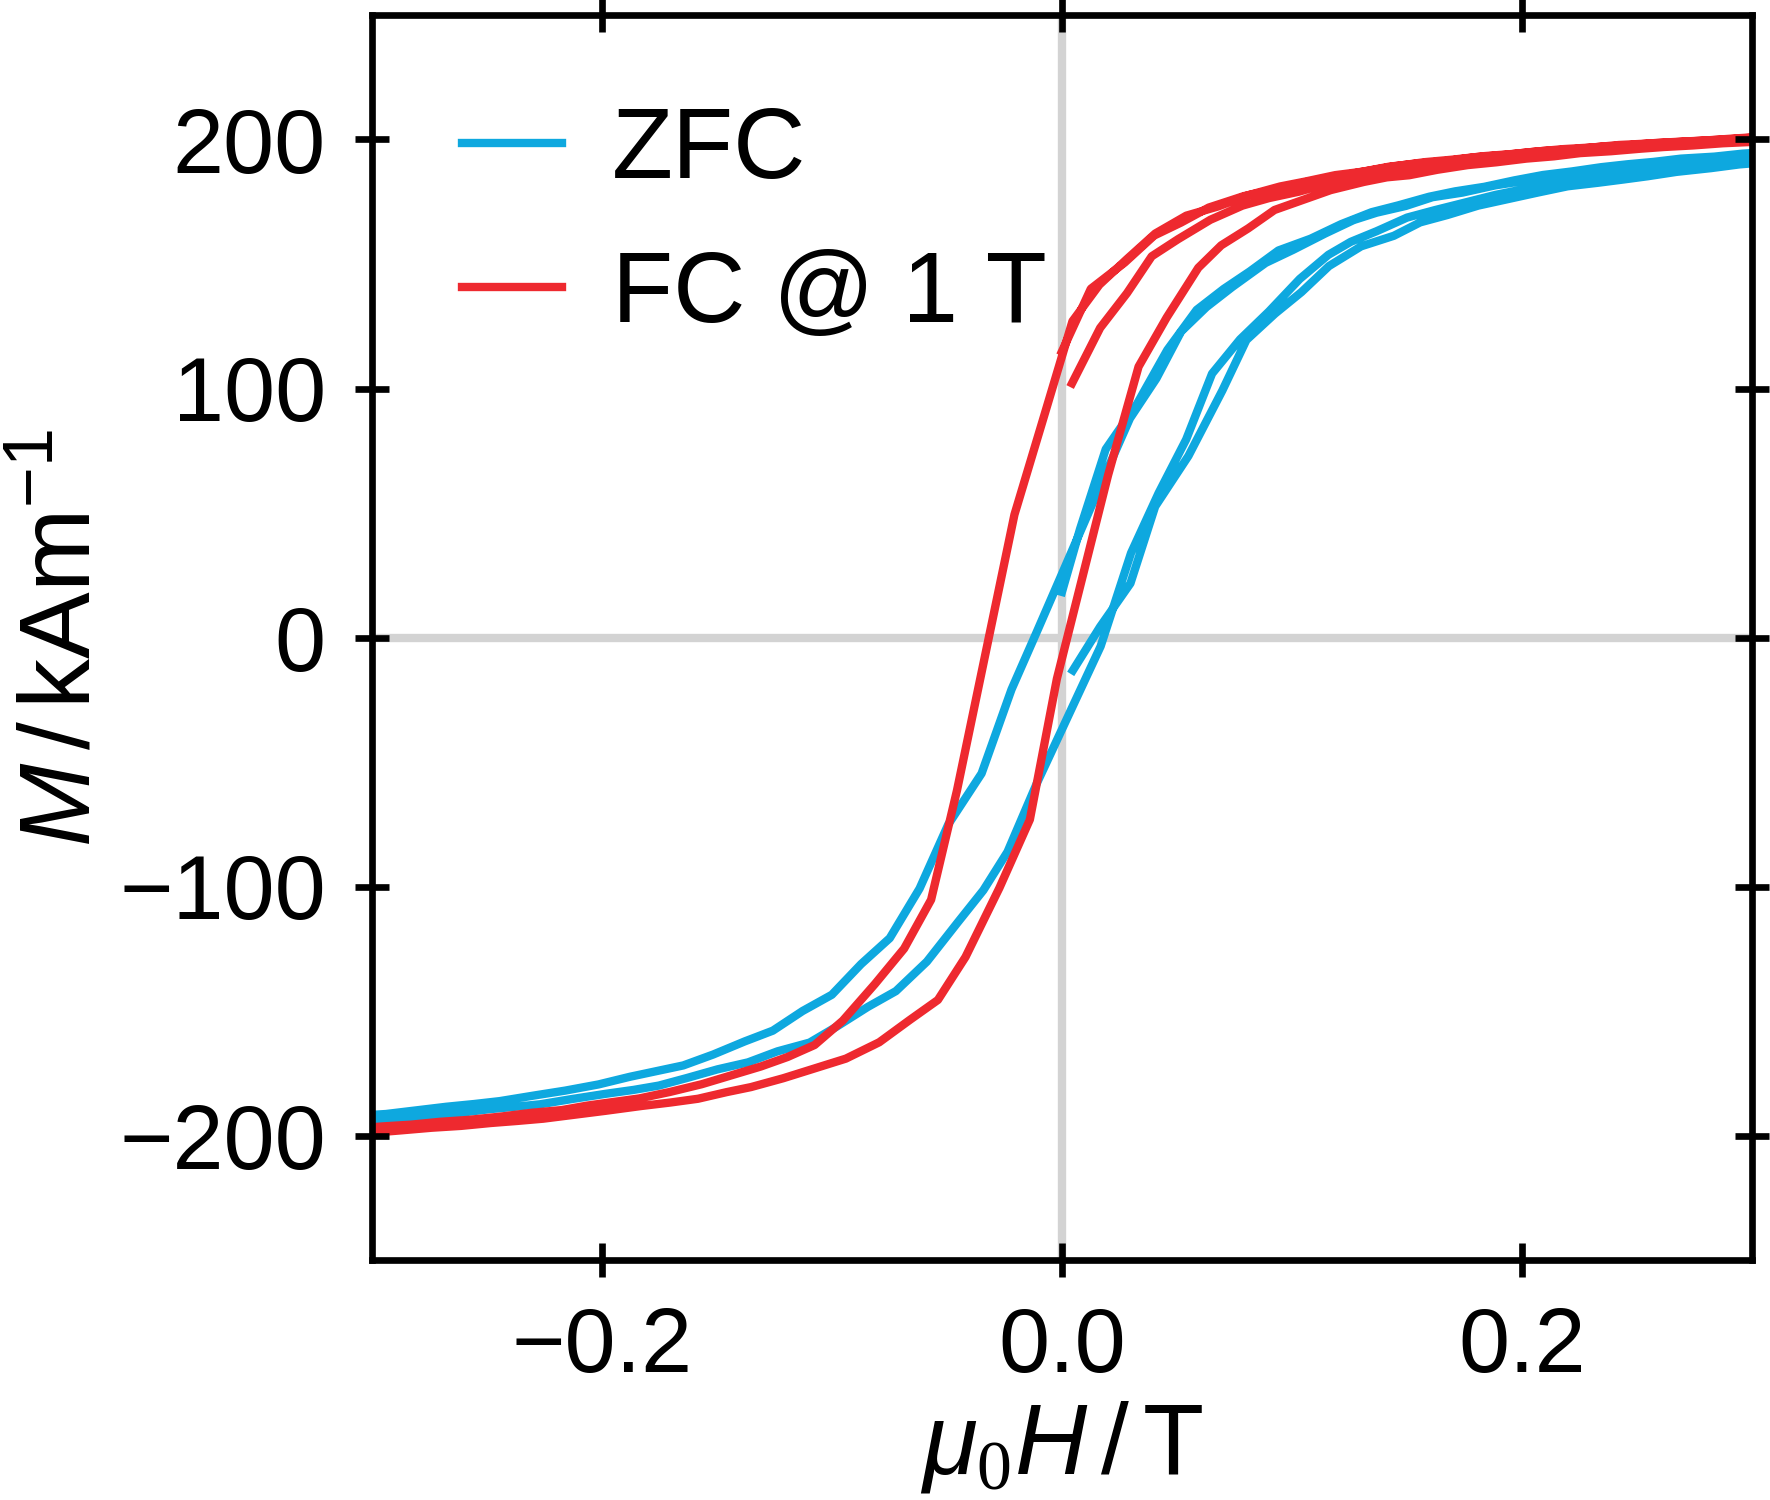
\includegraphics{looselyPackedNP_VSM_10K_IOS-11}
    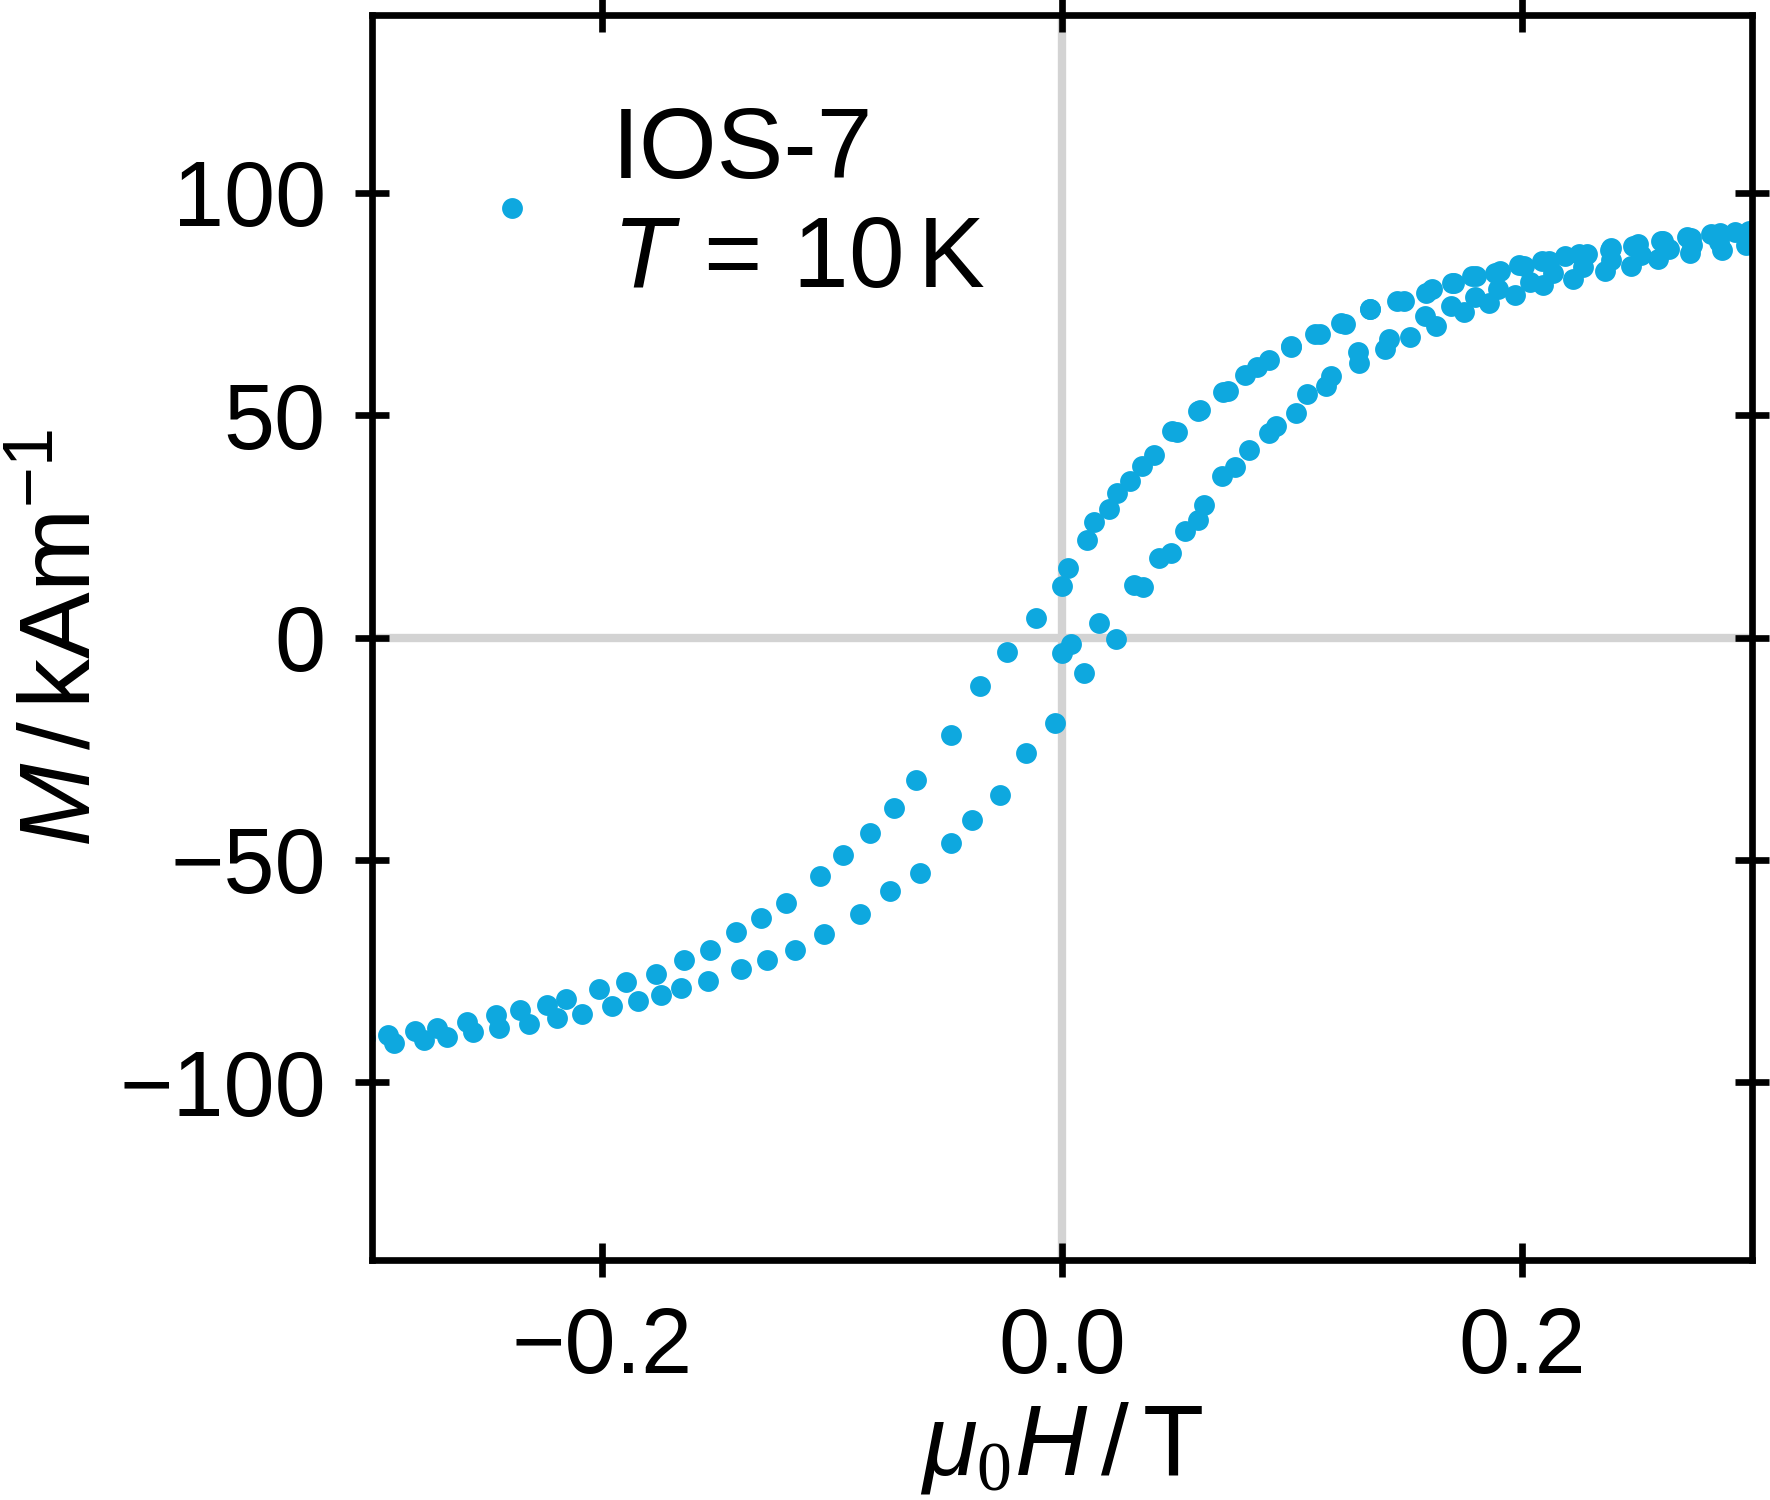
\includegraphics{looselyPackedNP_VSM_10K_IOS-7}
    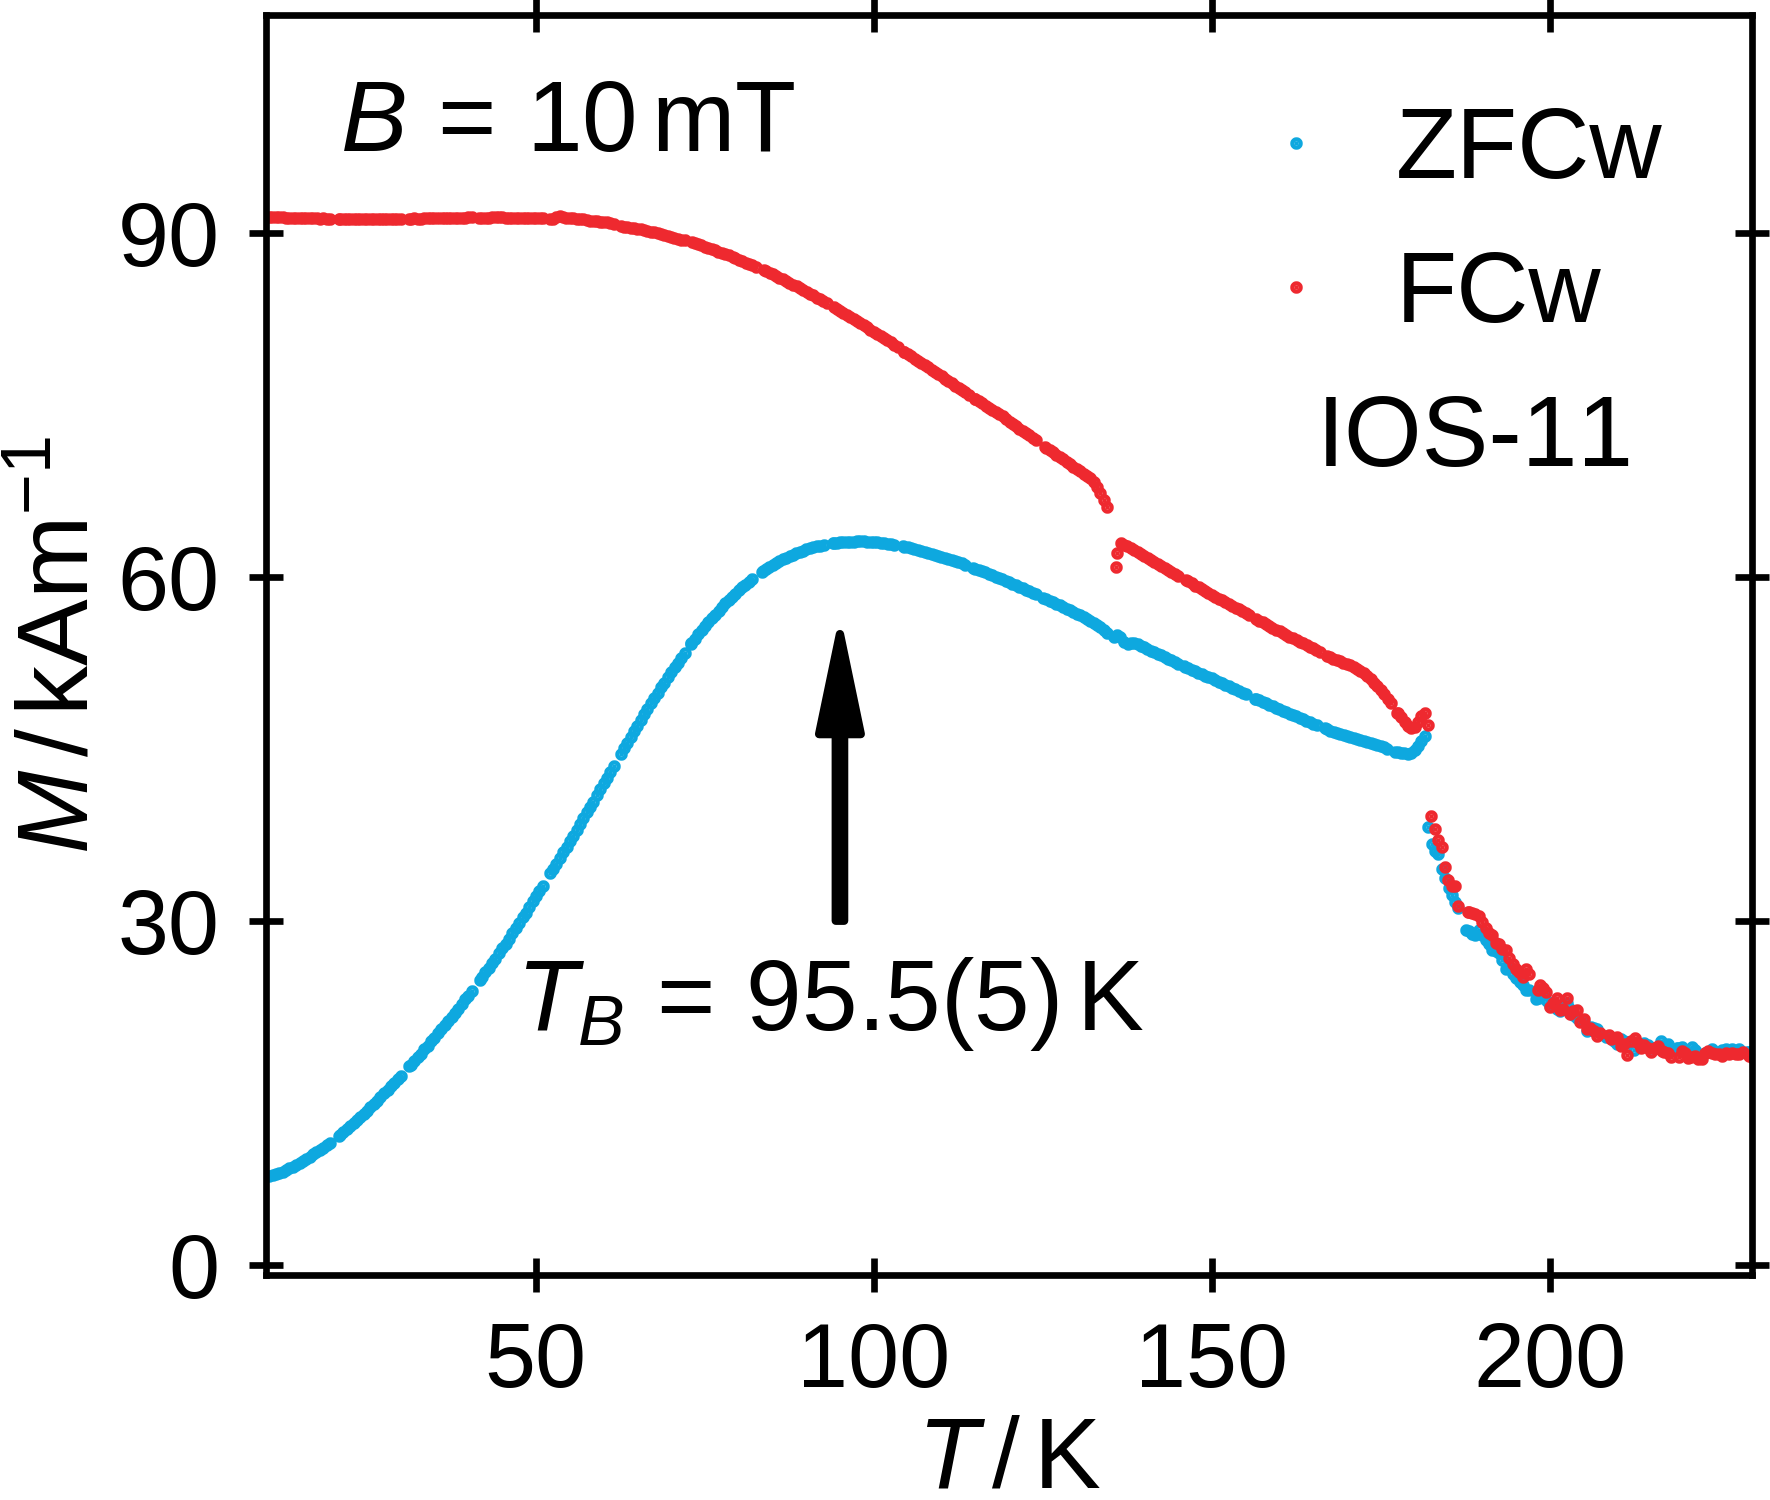
\includegraphics{looselyPackedNP_VSM_ZFC_FC_IOS-11}
    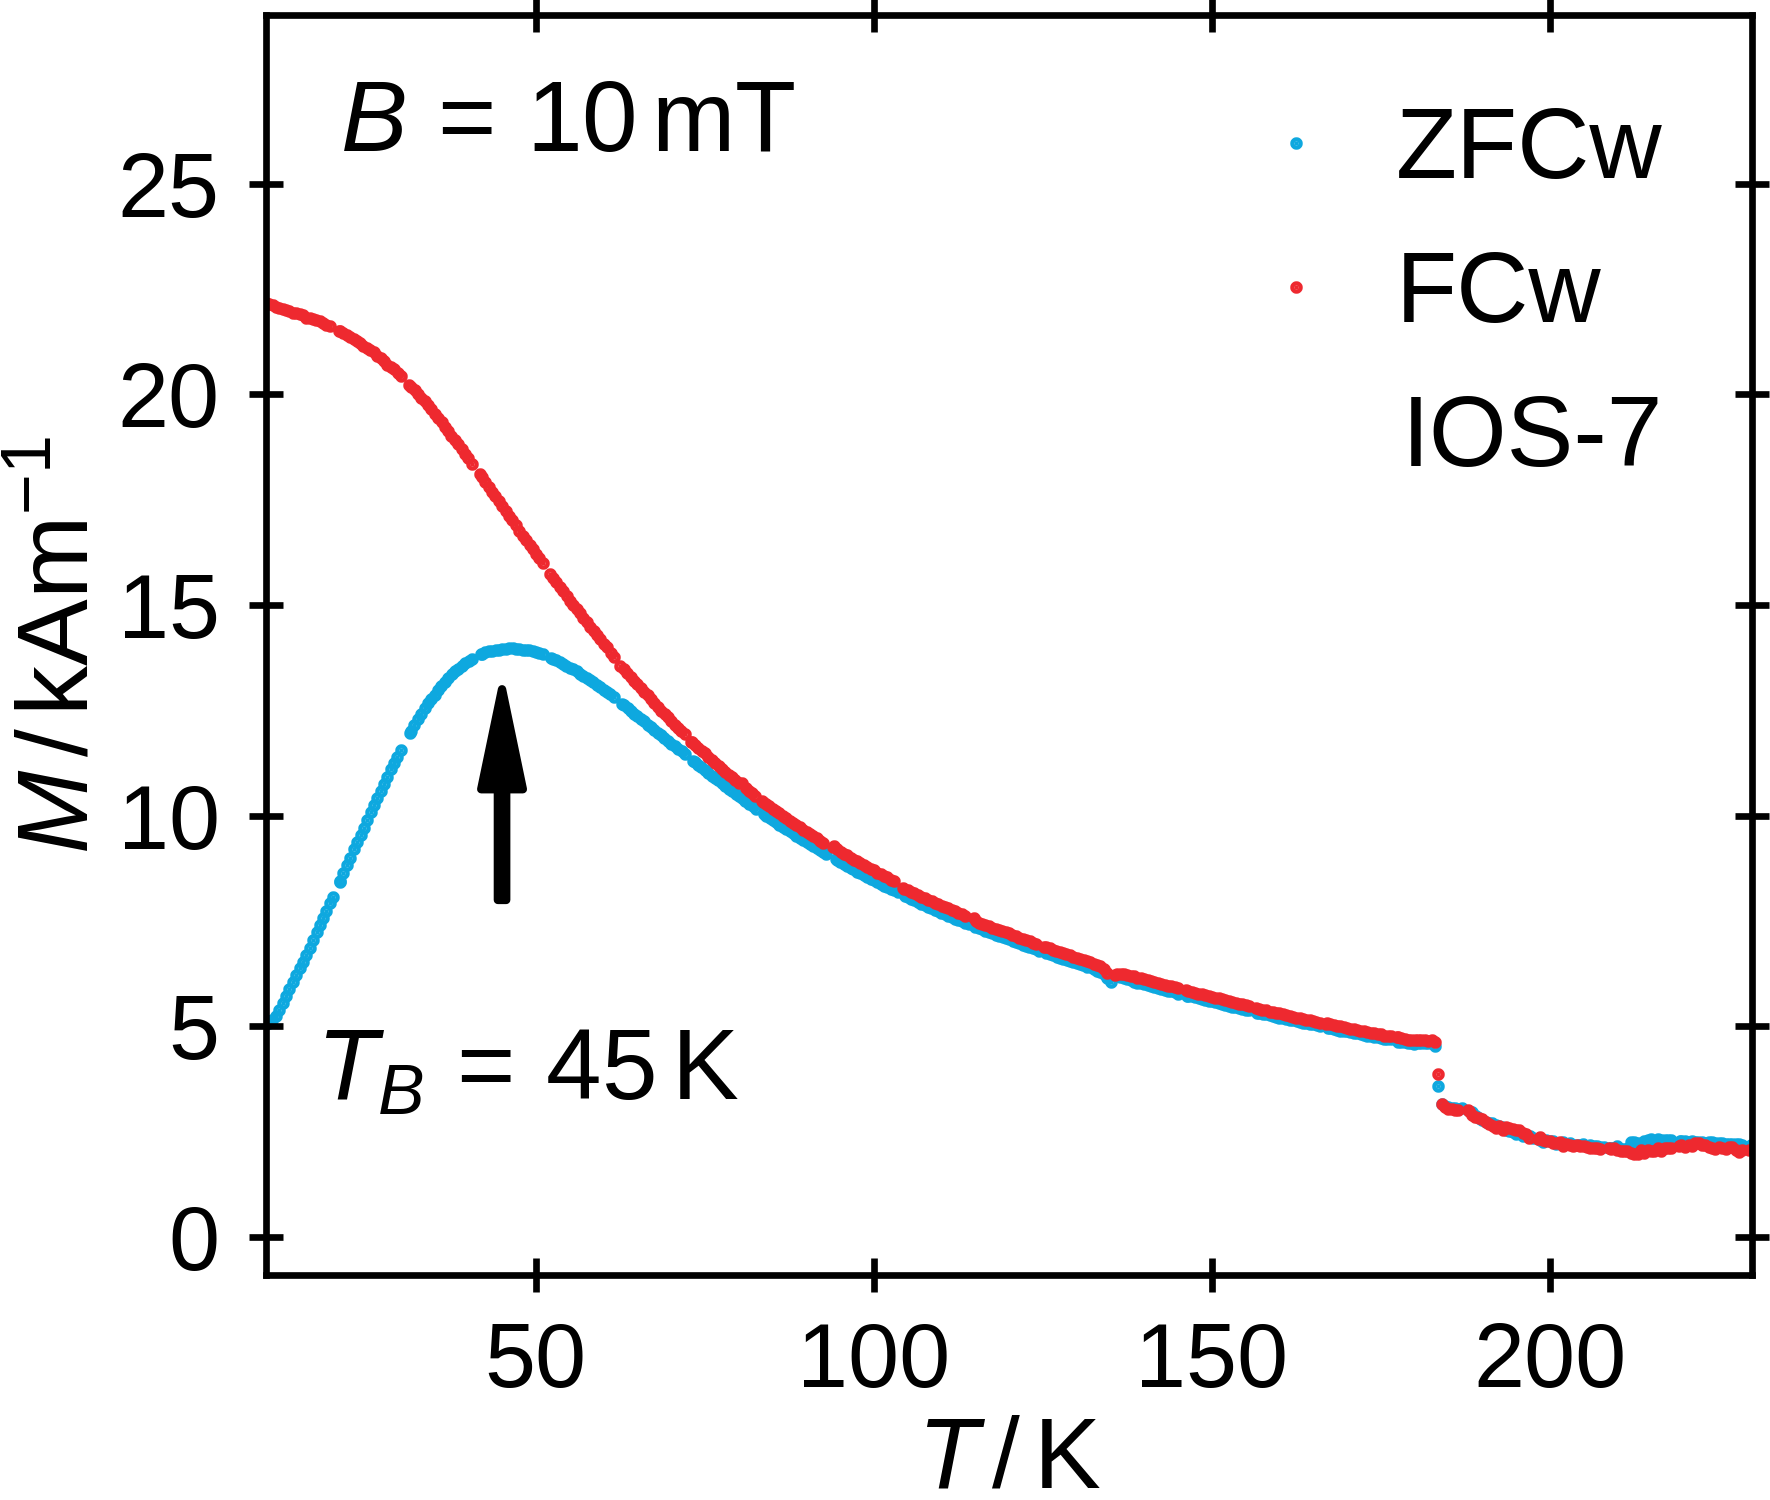
\includegraphics{looselyPackedNP_VSM_ZFC_FC_IOS-7}
    \caption{\label{fig:looselyPackedNP:nanoparticle:vsm10}Low-temperature hysteresis at $10 \unit{K}$ (upper) and temperature dependent magnetization measured at $10 \unit{mT}$ after cooling in zero-field and at a field of $10 \unit{mT}$ (lower) for IOS-11 (left) and IOS-7 (right).}
  \end{figure}
  At low temperatures the magnetization of IOS-11 and IOS-7 in \reffig{fig:looselyPackedNP:nanoparticle:vsm10} show a hysteretic behaviour, where IOS-11 has a coercive field of $40 \unit{mT}$ and IOS-7 a field of $25 \unit{mT}$.
  The temperature dependent curves furthermore show the blocking temperature of IOS-11 to be at $100 \unit{K}$ and for IOS-7 at $45 \unit{K}$.
  The smaller values observed for IOS-7 is connected to the larger population of small-sized nanoparticles, which even at low temperatures are more susceptible to thermal fluctuations.

\end{document}
